\begin{figure}[t]
    \centering
    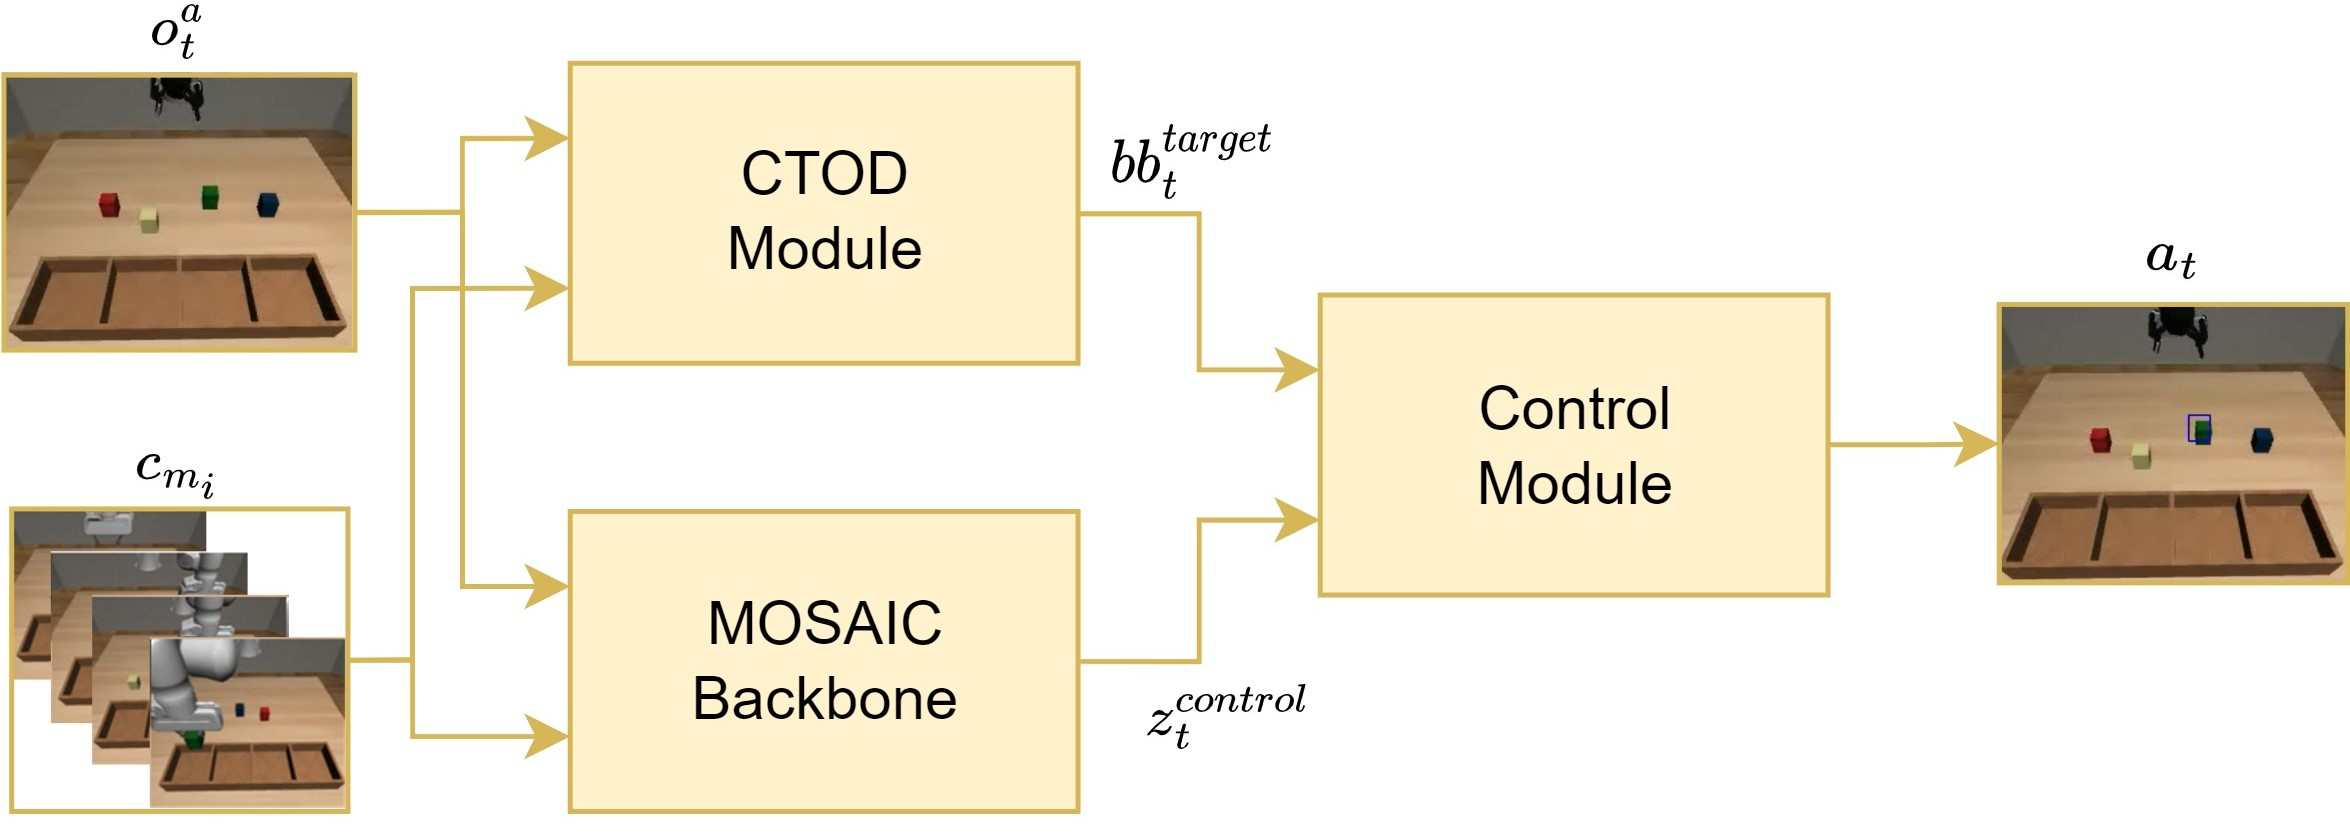
\includegraphics[width=0.9\textwidth]{figures/images/ch3/single_control_module.jpg}
    \caption{Proposed Single-Control Module Architecture. In contrast to the general architecture described in Figure \ref{fig:end_to_end_vs_modular}, the Command Analysis module is replaced by the CTOD module, which generates the bounding box related to the target object. The chosen backbone is the MOSAIC architecture \cite{mandi2022towards_more_generalizable_one_shot}. The control module is now informed by both low-level positional information ($bb^{target}_{t}$) and a control-oriented embedding ($z^{control}_{t}$), enabling it to make more informed decisions.}
    \label{fig:single_control_module}
\end{figure}
